\documentclass[11pt]{article}
\usepackage{amsmath}
\usepackage{amssymb}
\usepackage{amscd}
\usepackage{euler}

\usepackage{biblatex}
\addbibresource{bibliography.bib}

\usepackage{graphicx}
\graphicspath{ {./images/} }

\usepackage{amsthm}
\theoremstyle{definition}
\newtheorem{definition}{Definition}[section]
\newtheorem{theorem}{Theorem}[section]


\title{Neural network knowledge distillation in tensor networks}
\author{Dereck Piché}
\date{\today}
\theoremstyle{definition}


\begin{document}
\maketitle

\begin{abstract}
\end{abstract}

\section{Introduction}
TODO ctrl f R -> mathbb{R}
TODO fix spelling


\section{Knowledge Distillation}
Knowledge Distillation is a machine learning practice which involves
taking a trained model and using it's parameters to train another one.
The already trained model is referred to as the "teacher", and 
the model in which his "knowledge" is to be distilled is referred to as
the "student". While this is a relatively novel technique, there are 
already several distinct approaches introduced by researchers.
We used two of these approaches. Our inspiration for the distillation 
methodology was found in a a 2021 survey which resumed the emerging 
practice \cite{Gou_2021}.

\subsection{Response-Based Knowledge Distillation}
The first approach we used to look exclusively at the outputs
of the student and teacher. Now, we apply the logits
of our functions element-wise to the outputs and the softmax.
\begin{equation}
    softmax(v_i) = \frac{e^{v_i}}{\sum_{j}{e^{v_i}}}
\end{equation}
The softmax function's objective is to transform the logits
into probability distributions for the different classes.
We will now apply a loss function $L$ to these two functions.
Since we are trying to reduce the divergence between 
two distributions, we will use the Kullback-Leibler divergence loss
\begin{equation}
    KL(P, Q) = \frac{1}{n} \sum_i^n Q \frac{log_e(Q)}{log_e(P)}
\end{equation}
Here, $Q$ is the distribution we are aiming for and $P$ is the one we have.

\subsection{Layer-based approach}
The survey on Knowledge Distillation coined the term {\it Layer-based approach}.
Deep learning models work in layers of feature maps. It is hypothesized that
these different layers represent different layers of abstraction in the internal
representation of their input. 



\section{Tensor Networks}
Tensor Networks come from the study of quantum phenomena. They 
started being used recently as machine learning models. Tensor Networks
can be thought out as two things: a visual notation system and a 
set of methods for tensor manipulation. 

\subsection{Tensors}
Before explaining these two, we shall 
disambiguate the meaning of "tensor". In this report (and very often in the context
of machine learning), we use the word "tensor" to refer to the mathematical arrays
of arbitrary indices. Here, the number of indices is called the "order" of the 
tensor, meaning that vectors are simply tensors of order $1$ and matrices tensors 
of order $2$. 

\subsection{Contraction}
At the heart of tensor networks is the {\it contraction} operation.
Tensor Networks are used to compute a larger network by "contracting" several
smaller tensors over chosen indices. A "contraction" is simply an operation 
where we sum over indices. For example, the contraction of $A_{ijk}$ and 
$B_{ijk}$ on index $j$ will produce the tensor $C_{ik} = \sum_{j} A_{ijk} B_{ijk}$.
Evidently, the two indices present in a contraction must be of the same size.

\subsection{Tensor Networks as a graphical system of notation}
The principal motivation behind the creation of Tensor Networks 
to compute or approximate large tensors {\it contracting} several
smaller tensors over chosen indices. This is all well and good until 
our conventional summation notation begins overclocking our primal brains.
So, in order to make the manipulation of these network of tensors, mathematicians
created a notational system. Tensors are represented as nodes where each 
vertex connected to the node represents one of the tensor's indices. 
If a vertex connects two nodes, it means that the indices shall be contracted 
in order to produce the post-contraction tensor. It should be evident that
by the definitions above, no node (tensor) is completely isolated in a tensor network,
as it would be completely purposeless. The shape of the post-contraction tensor 
can be easily visually identified, since it is found in the unconnected vertices.
A simple tensor network can be found in figure \ref{fig:tensor_net}.

\subsection{Tensor Network Methods}
The term {\it Tensor Network Methods} is used to refer to, you guessed it, the methods.
There are several architectures of Tensor Networks that are frequently used, such 
as the {\it Matrix Product State (MPS)}, the {\it Tenso}

\begin{figure}[h]
\centering
\caption{Simple tensor network illustrating the notation.}
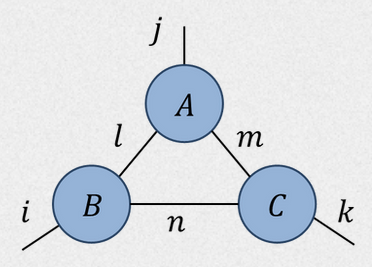
\includegraphics[width=0.5\textwidth]{images/2023-03-21-10-22-39.png}
\label{fig:tensor_net}
\end{figure}

\section{Kernel}

Consider an input vector $x \in R^d$. Let $\phi(x) : R \mapsto R^{d_{\phi}}$.  
Then, let us take the tensor product of apply $\phi(x)$ applied 
to every element of the vector $x$.
\begin{equation}
    \Phi(x) = \phi(x_1) \otimes  \phi(x_2) 
                \otimes (\dots) \phi(x_d)
\end{equation}
We obtain a tensor $\Phi(x)$, of which the sum of it's element 
contain the basis of a space of products of the elements of the transformed
elements of $\phi(x)$.

In order to reduce the abstractness of this statement, we can take say
that $\otimes$ refers to the Kronecker Product.

\subsection{Multilinear feature map}
In this project, we attributed a particular importance to the local feature map
\begin{equation}
    \phi^*(x) = 
    \begin{bmatrix}
        1 \\
        x
    \end{bmatrix}
\end{equation}
With, this particular transformation, the Kronecker Product gives us a global feature map
$\Phi(x)$ which is a tensor where each element is a basis of the 
space of multilinear functions on the elements of the vector $x$. Here, the 
order or shape of the tensor is superfluous and gives no theoretical advantage.

\subsection{Linear Combinations}
Now, the question is how do we use $\Phi(x)$, how does it become useful? 
Well, it becomes useful when we take a linear map of it's elements. Let our $\Phi(x)$ be an 
arbitrarily shaped tensor of $d_{\Phi}$ dimensions. The final form of our 
function $f(x)$ will be
\begin{equation}
    f(x) = \sum_{i}^{d_{\Phi}} \theta_i [\Phi(x)]_i
\end{equation}
Now, we have a function that can, under some choice of transformation
$\phi$, become extremely expressive. For our particular local feature map 
$\phi^*$, it can represent any multililinear function  of the input vector $x$. 
We shall represent linear combinations of $\Phi(x)$ by $T\Phi(x)$.

\section{Using The Matrix Product State Tensor Network}
In this project, we used the {\it Matrix Product State} (MPS) tensor network to 
approximate the function $T  \Phi(x)$. Here, this function is computed by contracting 
a Tensor Network. Before the contraction, some of the elements of the tensors in the 
tensor network are set by applying the mapping $\phi^*(x)$.

\subsection{Single MPS}
TODO add info to this!
How does the Matrix Product State decomposition work? What does it look like?.
Suppose we have a Tensor of the form $T$.
A single MPS network can reproduce functions of the form 
\[  
    f(x) = T \left( 
            \phi(x_1) \otimes 
            \phi(x_2) \otimes 
            \dots \otimes 
            \phi(x_N) = T \Phi(x)
        \right)
\]
We can rewrite this function as
\[  
    g ( f ( x ) )
\]

\subsection{Composition of MPS}
When we use the $ \begin{bmatrix} 1 \\ x \end{bmatrix} $ local feature map, a single
MPS can only express multilinear functions of $x$. It would be practical 
for our model to be able to express multipolynomial functions up to a certain degree $z$.
In order to do this, we will require a composition of two MPS. The 2-MPS, when contracted,
shall approximate the function
\[  
    g' \circ f \circ g \circ f (x)
\]
We will show in a proof that this composed function can express any polynomial function of degree $z$.

\subsubsection{Proof of expressivity}


\begin{equation} \label{composition_graph}
    \begin{CD}
        @. X \in R^d 
        @>f>> Y_1 \in R^{2^d}
        @>g>> Y_2 \in R^{zd} 
        @>f>> Y_3 \in R^{2^{zd}}
        @>g'>> Y_4 \in R
    \end{CD}
\end{equation}


\begin{definition}[Multilinear polynomial]
    A multilinear polynomial is a function $f: R^n \mapsto R$ of the form
    \begin{equation}
        f(x) = T \cdot \left( 
            \begin{bmatrix} 1 \\ x_1 \end{bmatrix} \otimes 
            \begin{bmatrix} 1 \\ x_2 \end{bmatrix} \otimes 
            \dots \otimes 
            \begin{bmatrix} 1 \\ x_d \end{bmatrix}
        \right)
    \end{equation}
    Where $T \in R^{p \times R^n }$. In other words, a multilinear polynomial is a polynomial that is linear if  $\forall x_i$ then the polynomial is linear if we fix every variable except $x_i$.
\end{definition}

\begin{definition}[$v_i$-variate]
Function of the variables of the vector $v$. (Each element of $v$ is considered as a variable).
\end{definition}


\begin{theorem}
    Any polynomial function $\Gamma: R^d \mapsto R$ of degree $z$ can be expressed by the composition
    as the composition of functions illustrated in \ref{composition_graph}.
\end{theorem}

\begin{proof}
Let the function $g$ in \ref{composition_graph} be defined such that

\begin{equation}
    g(f(x))
    = 
    \begin{bmatrix}
        \textit{repeated $z$ times} 
        \begin{cases}
            x_1 &  \\
            (\dots) & \\
            x_1 & 
        \end{cases} \\
        \textit{repeated $z$ times} 

        \begin{cases}
            x_2 &  \\
            (\dots) & \\
            x_2 & 
        \end{cases} \\
        (\dots) \\
        \textit{repeated $z$ times} 
        \begin{cases}
            x_n &  \\
            (\dots) & \\
            x_n & 
        \end{cases} \\
    \end{bmatrix}
\end{equation}
We can rewrite this vector as 

\begin{equation} \label{lambda}
    g(f(x))
    = 
    \begin{bmatrix}
        \varepsilon_{1, 1} \\
        (\dots) \\
        \varepsilon_{1, z} \\
        \varepsilon_{2, 1} \\
        (\dots) \\
        \varepsilon_{2, z} \\
        (\dots) \\
        \varepsilon_{d, z} 
    \end{bmatrix}
    = \lambda
\end{equation}

Let $Z$ be the space of $x_i$-variate polynomial functions 
of degree $\leq z$. By definition, every monomial of $\zeta \in Z$ is of the form
\begin{equation}
    x_{1}^{k_1}x_{2}^{k_2}(\dots)x_{d}^{k_d}
\end{equation}
, where $\sum k_i \leq z$. \\
However, for every set $\{k_1, k_2, (\dots), k_d\}$ meeting this condition,
we can rewrite the monomial as
\begin{equation}
    \left( \prod_{i_1=1}^{k_1}\varepsilon_{1, i_1} \right)
    \left( \prod_{i_2=1}^{k_2}\varepsilon_{2, i_2} \right)
    \left( \dots \right)
    \left( \prod_{i_d=1}^{k_d}\varepsilon_{d, i_d} \right)
\end{equation}
by using the elements of $\lambda$ from equation \eqref{lambda}.

However, we can clearly see that this term is a multilinear 
monomial of the variables in $\lambda$. This implies that
$f(\lambda*)$ returns a basis-vector of $x_i$-variate polynomial 
function of degree $\leq z$.

In other words, 
\begin{equation}
    \xi \left( x, \Theta \right) =
        M
        \left(
            f
            \left(
                M
                \left(
                    f
                    \left(
                        x 
                    \right),
                    \Theta^*
                \right)
            \right),
            \Theta
        \right)
\end{equation}
can express any $x_i$-variate polynomial function of degree $\leq z$ under
fixed $\Theta$.

\end{proof}

\subsection{Patching of MPS (experimental)}






\section{Methodology}
The experiments done for the projet were programmed using Python. 
Now, evidently, using Python alone was not possible. The big 
deep learning library we used was Pytorch, as is common in machine learning today.
However, it does not provide many tools to train and build Tensor Networks. 
We thus used TorchMPS \cite{torchmps}, a library built using Pytorch for the creation 
and training of learning Matrix Product State tensor networks.

\paragraph{Learning rate} ${}$ \\
We used the very standard learning rate of $0.01$. This is the learning rate
used by {\it Keras}.

\paragraph{Model size} ${}$ \\

\paragraph{Approach to the results}
As a matter of scientific integrity, we have chosen to show the 
results even if they are heavily disappointing. Not doing so 
can result in certain statistical biases which can be avoided.

Learning rate for neural network: 0.01
Learning rate for MPS: 1e-3 = 0.001
Nb of normal epochs: 25
Nb of gaussian epochs: 5


\section{Results}
\subsection{Training the single MPS}
TODO: ALL THE FOLLOWING WITH AND WITHOUT OUR CUSTOM FEATURE MAP (sin cos)

TODO: train for baseline
train batch loss MPS:
valid loss MPS:

TODO: train with teacher
horizontal bar for teacher:
train batch loss MPS:
valid loss MPS:

TODO: comparison through epochs
valid loss distill MPS:
valid loss base MPS:

\subsection{Training the hidden-layered MPS}
TODO: 
train batch loss 2-MPS:
valid loss 2-MPS:




TODO: 
horizontal bar for teacher
train batch loss 2-MPS:
valid loss 2-MPS:

TODO: 
valid loss distill MPS
valid loss base MPS

\subsection{Comparison}
TODO: 
valid loss 2-MPS
valid loss base MPS

\subsection{Training the patch-MPS}
TODO: Explain why the training failed.


\section{Analysis}




\section{Conclusion}



\subsection{Further Exploration}
TODO talk about capturing locality in the mappings
TODO talk about capturing locality in general with tensors

\printbibliography

\end{document}




































Person 1: *waiving vigorously
    HELLO CAN YOU SEE ME!
    HEYYY! 

Person 2:
    For the last time, they can't see you... 
    YOU'RE OUTSIDE THE DOCUMENT DELIMITERS!

Person 1: 
    I feel so alone... 

Person 2: 
    Bro I'm here...